% Chapter Template

\chapter{Set cover problems} % Main chapter title

\label{Chapter1} % Change X to a consecutive number; for referencing this chapter elsewhere, use \ref{ChapterX}

To set cover problem είναι ένα κλασικό πρόβλημα στον τομέα της συνδυαστικής βελτιστοποίησης και της θεωρίας υπολογιστών, η μελέτη του οποίου έχει οδηγήσει στην ανάπτυξη θεμελιωδών τεχνικών στο πεδίο των προσεγγιστικών αλγορίθμων. Λόγω της γενικής του διατύπωσης βρίσκει εφαρμογές σε μια ευρεία γκάμα προβλημάτων.
%----------------------------------------------------------------------------------------
%	SECTION 1
%----------------------------------------------------------------------------------------

\section{Διατύπωση}
Το πρόβλημα μπορεί να διατυπωθεί με διάφορους τρόπους, είτε ως πρόβλημα βελτιστοποίησης όπου ζητείται ο ελάχιστος αριθμός υποσυνόλων ή, αν έχει ανατεθεί συνάρτηση κόστους στα υποσύνολα, ζητείται το σύνολο με το ελάχιστο κόστος, είτε ως πρόβλημα απόφασης. 

%-----------------------------------
%	SUBSECTION 1
%-----------------------------------

\subsubsection{Απλή διατύπωση}
Δεδομένου ενός σύμπαντος $U$ αποτελούμενο από $n$ στοιχεία κι ενός συνόλου από υποσύνολα του $U$, $S = \{S_1,...,S_k\}$ τέτοια ώστε η ένωσή τους να είναι το σύνολο $U$, βρες το ελάχιστο υποσύνολο του $S$ που καλύπτει όλα τα στοιχεία του $U$.

\subsubsection{Με συνάρτηση κόστους}
Δεδομένου ενός σύμπαντος $U$ αποτελούμενο από $n$ στοιχεία, μιας συλλογής από υποσύνολα του $U$, $S = {S_1,...,S_k}$, και μίας συνάρτησης κόστους $c : S \rightarrow {\boldsymbol{Q}^+}$, βρες το υποσύνολο του $S$ με το ελάχιστο κόστος που καλύπτει όλα τα στοιχεία του $U$.

\subsubsection{Πρόβλημα απόφασης}
Δεδομένου ενός σύμπαντος $U$ αποτελούμενο από $n$ στοιχεία, μιας συλλογής από υποσύνολα του $U$, $S = {S_1,...,S_k}$, και ενός ακεραίου $k$, αποφάσισε αν υπάρχει υποσύνολο του $S$ με το πολύ $k$ στοιχεία που καλύπτει όλα τα στοιχεία του $U$.

\subsubsection{Παράδειγμα}
Έστω το σύμπαν $U = \{1, 2, 3, 4 ,5\}$ και η συλλογή από υποσύνολα του $S=\{\{1,2,3\},\{2,4\},\{3,4\},\{4,5\}\}
$. Η ένωση των στοιχείων του $S$ καλύπτει το $U$. H ελάχιστη συλλογή υποσυνόλων του $S$ που καλύπτει το $U$ είναι τα : $\{\{1,2,3\},\{4,5\}\}$.

\begin{figure}[H]
\caption{Set cover example}
\centering
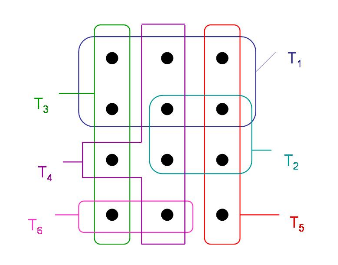
\includegraphics[width=0.4\textwidth]{Figures/set_cover.png}\centering
\end{figure}

Το ελάχιστο set cover είναι το σύνολο $S' = \{T_3, T_4, T_5\}$

\begin{figure}[H]
\caption{Minimum set cover example}
\centering
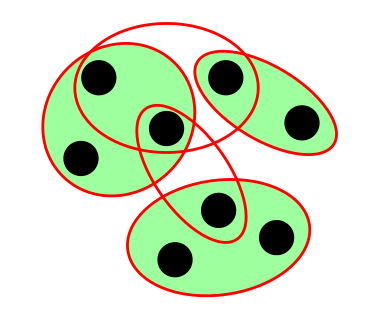
\includegraphics[width=0.4\textwidth]{Figures/min_set_cover.png}\centering
\end{figure}

%----------------------------------------------------------------------------------------
%	SECTION 2
%----------------------------------------------------------------------------------------

\section{NP-πληρότητα}

To set cover decision problem είναι ένα από τα 21 NP-πλήρης προβλήματα του Karp που αποδείχθηκε ότι είναι NP-πλήρης το 1972. Αυτό σημαίνει ότι ανήκει στην κλάση NP δηλαδή δεδομένου ενός σύμπαντος $U$, μιας συλλογής $S$ από υποσύνολα, ενός ακεραίου $k$ και μίας λύσης $S'$ η λύση αυτή μπορεί να επαληθευτεί σε πολυωνυμικό χρόνο όσον αφορά το μέγεθος των στοιχείων της εισόδου. Επίσης ανήκει και στην κλάση NP-hard. Αυτό οδήγησε στην ανάπτυξη προσεγγιστικών αλγορίθμων για την επίλυση του προβλήματος αυτού.


\section{Λύσεις}

\subsection{Πρόβλημα ακέραιου προγραμματισμού}

Το minimum set cover problem μπορεί να διατυπωθεί ως το ακόλουθο πρόβλημα ακέραιου προγραμματισμού

$$min\{\displaystyle\sum_{S\in{\mathcal{S}}} x_S\}$$ 
\centerline{subject to}
$$\displaystyle\sum_{S:e\in{\mathcal{S}}} x_S \geq{1}, \quad \forall e \in{\mathcal{U}}$$
$$ x_S \in{\{0, 1\}}$$

Επειδή το πρόβλημα ακέραιου προγραμματισμού είναι NP-hard χαλαρώνουμε τους περιορισμούς του προβλήματος για το $x_S$ και το ανάγουμε σε πρόβλημα γραμμικού προγραμματισμού το οποίο λύνεται σε πολυωνυμικό χρόνο. Έτσι καταλήγουμε στο πρόβλημα:

$$min\{\displaystyle\sum_{S\in{\mathcal{S}}} x_S\}$$ 
\centerline{subject to}
$$\displaystyle\sum_{S:e\in{\mathcal{S}}} x_S \geq{1}, \quad \forall e \in{\mathcal{U}}$$
$$ x_S \in{[0, 1]}$$

Επειδή το integrality gap αυτού του προβλήματος είναι το πολύ $\log{n}$ η χαλάρωση του δίνει factor-$\log{n}$ προσεγγιστικό αλγόριθμο.
Αν κάθε στοιχείο εμφανίζεται το πολύ σε ${\mathcal{F}}$ τότε μπορεί να βρεθεί λύση σε πολυωνυμικό χρόνο η οποία προσεγγίζει το βέλτιστο με παράγοντα ${\mathcal{F}}$ χρησιμοποιώντας το πρόβλημα γραμμικού προγραμματισμού.

\subsection{Άπληστος αλγόριθμος} 

Υπάρχει και ένας άπληστος αλγόριθμος για προσέγγιση σε πολυωνυμικό χρόνο ο οποίος διαλέγει τα σύνολα με έναν μόνο κανόνα: σε κάθε στάδιο διαλέγει το σύνολο που περιέχει τον μεγαλύτερο αριθμό από ακάλυπτα στοιχεία.

Αλγόριθμος:
\begin{enumerate}
\item $ C \leftarrow \emptyset$
\item While $ C \neq {\mathcal{U}} $ do
\begin{enumerate}
\item Find the set whose cost effectiveness is smallest, say $S_i$. \\
			Let $a = \frac{c(S_i)}{|S_i-C|}$. \\
			Pick $S_i$ and $\forall e \in{S_i - C}$, set $price(e) = a$.
\item $C \leftarrow S_i \cup C$
\end{enumerate}
\item Output $C$
\end{enumerate}

\section{Hitting set}
Το πρόβλημα set cover είναι ισοδύναμο με το πρόβλημα hitting set. Αν σε έναν διμερή γράφο το ένα σύνολο κόμβων ${\mathcal{U}}$ αντιπροσωπεύει τα υποσύνολα ${\mathcal{S}}$ του σύμπαντος, το άλλο σύνολο κόμβων ${\mathcal{V}}$ αντιπροσωπεύει τα στοιχεία του σύμπαντος και οι ακμές αντιπροσωπεύουν την συμπερίληψη ενός στοιχείου σε ένα σύνολο τότε βρίσκουμε τον ελάχιστο αριθμό κόμβων του συνόλου ${\mathcal{U}}$ που καλύπτει όλους τους κόμβους του συνόλου ${\mathcal{V}}$.

\section{Εφαρμογές}
IBM finds computer viruses (wikipedia) 
elements- 5000 known viruses 
sets- 9000 substrings of 20 or more consecutive bytes from viruses, not found in ‘good’ code 
A set cover of 180 was found.  It suffices to search 
for these 180 substrings to verify the existence of 
known computer viruses. 
Another example:  Consider General Motors needs to 
buy a certain amount of varied supplies and there are 
suppliers that offer various deals for different combina
tions of materials (Supplier A: 2 tons of steel + 500 tiles 
for \$x; Supplier B: 1 ton of steel + 2000 tiles for \$y; etc.).  You could use set covering to find the best way to 
get all the materials while minimizing cost